\section{Evaluation} \label{sec:automaticeval}

\subsection{Automatic evaluation}

Using \puse~learned as described in Section~\ref{sec:learning} and running our algorithm 100 times and execute the automatic evaluation with the automatic metrics given by~\cite{} in the ASGRE-challenge.
They calculate minimality, defined as the proportion of descriptions produced by a system
that are maximally brief, as per the original definition in Dale (1989). The Dice coefficient, used to compare the description produced by a system to the human-produced description on the same input domain. %Dice is estimated
MASI, a version of the Jaccard similarity coefficient proposed
by Passonneau (2006) which multiplies the similarity value by a monotonicity coefficient, biasing
the measure towards those cases where DS and
DH have an empty set difference. Intuitively, this
means that those system-produced descriptions are
preferred which do not include attributes that are
omitted by a human. Thus, two of our intrinsic measures assess Humanlikeness (Dice and MASI), while
Minimality reflects the extent to which an algorithm
conforms to brevity, one of the principles that has
emerged from the ASGRE literature.
Since our system is capable of give a lot of RE for the same domain, we also did another comparison taking into account the 20 first RE that the system produced named SYS\_Furniture\_20 and SYS\_People\_20 in table~\ref{Tabla_sis_1_20}, and when in those 20 is the given for a human we choise this one, we obtain the following results:

ROMI: AGREGAR RESULTADOS DE GRAPH A LA TABLA SIGUIENTE Y AGREGAR GRAFICOS

\begin{table}[h!]
\begin{center}
\begin{tabular}{|l|c|c|c|c|}
\hline
%Figure & Model \puse &  Learning \puse & Random \puse &  Uniform \puse \\
	 	& 	DICE		&	MASI	&	A\_ACCURACY	&MINIMALITY	\\
\hline
GRAPH Furniture	& 	.80 		&	.59	&	.48		&	.0 	\\
GRAPH People 	& 	.72		&	.48	&	.28		&	.0	\\
\hline
SYS\_Furniture	&	.79		&	.58	&	.43		&	.01	\\
SYS\_People	&	.65		&	.37	&	.19		&	.0	\\
\hline
SYS\_Furniture\_20	&	.87		&	.75  	&	.65		&	.01	\\
SYS\_People\_20	&	.81		&	.68	&	.60		&	.01	\\
\hline
\end{tabular}
\caption{Comparison GRAPH and our system the more frequent and the first 20}
\label{Tabla_sis_1_20}
\end{center}
\end{table}

Our results are comparable with the best results of the ASGRE challenge, but we also will show in the Section~\ref{sec:evaluation} that the RE generated by te system are more prefered than the humans ones.

\begin{table}[h!]
\begin{center}
\begin{tabular}{|l|c|c|}
\hline
		& Count		& Percentage\\
\hline
It is not RE	&	11	&	13.75\% \\
%		&	37	&	46.25\% \\
Contains ``other''	&	6	&	7.50\% \\
SYS does not generated the RE in 100 runs	&	8	&	10.00\% \\
SYS generated but not with higuer frequency	&	18	&	22.5\% \\
\hline
\end{tabular}
\caption{Error clasification of People}
\label{error-people}
\end{center}
\end{table}


\begin{table}[h!]
\begin{center}
\begin{tabular}{|l|c|c|}
\hline
			& Count		& Percentage\\
\hline
NO ES RE		&	4	&	5.88\% \\
Contains ``other''	&	6	&	8.82\% \\
SYS does not generated the RE in 100 runs	&	17	&	25.00\% \\
SYS generated but not with higuer frequency	&	28	&	41.18\% \\
%BIEN			&	13	&	19.12\% \\

\hline
\end{tabular}
\caption{Error clasification of Furniture}
\label{error-furniture}
\end{center}
\end{table}
ROMI: AGREGAR UNA TABLA DE CLASIFICACION DE ERRORES

\subsection{Human evaluation} \label{sec:evaluation}

We aisle the RE that our system gives another RE with more frequency it is that not coincides with the one given by the human in the corpus, and with those realize a human evaluation in order to see if the RE produced by the system are prefered by human than the RE produced by humans. Two judges were asked by each pair of RE.

We have 43 pictures of furniture (from 80) and 55 pictures of people (from 68), for wach of them we manually realize the referring expressions (including the properties given as results by our algorithm) and ask people to evaluate which one is a RE it is that univocally identifies the target object and wich one is better in sense that will be more usefull for a human who is not seeing the red box to identify the object. For do it we prepare a webpage with each of the pictures and 2 choices randomly ordered human and system RE. Out goal is to try to show if RE produced by our system are at less as good as the produced by human, and also we will show that they are even better.

%\begin{table}[h!]
%\begin{center}
%\begin{tabular}{|c|c|c|c|}
%\hline
%           & Agree in & Not agree & Total\\
%\hline 
%Furniture & 25       & 18        & 43 \\
%People    & 25       & 30        & 55 \\
%Total     & 50       & 48        & 98 \\
%\hline
%\end{tabular}
%\caption{Agree between judges} 
%\label{agree-judges}
%\end{center}
%\end{table}

%esta tabla no ayuda...no se que decir, no se como justificar que no coincidan...
%In the Table~\ref{agree-judges} we can see that the both judges choice the same RE 25 times for Furniture and 25 times for People, 

\begin{table}[h!]
\begin{center}
\begin{tabular}{|c|c|c|c|c|}
\hline
Judge    & Human choice & System choice  & Human choice & System choice \\
	 &    Furniture &    Furniture   &    People    &    People \\
\hline 
Judge1   & .23       & .77      & .45  & .55  \\
Judge2   & .26       & .73      & .41  & .59  \\
\hline
\end{tabular}
\caption{Porcentage of system versus human selected choices for each judge} 
\label{system-versus-human}
\end{center}
\end{table}

In the Table~\ref{system-versus-human} you can see the judges selected more the RE generated by our system than the human RE.

%\begin{table}[h!]
%\begin{center}
%\begin{tabular}{|c|c|c|c|}
%\hline
%Judge    & Human choice & System choice & Total\\
%\hline 
%Judge1 & 25       & 30        & 55 \\
%Judge2    & 23       & 32        & 55 \\
%\hline
%\end{tabular}
%\caption{System versus human selected choice for People} 
%\label{system-versus-human-people}
%\end{center}
%\end{table}

%In the case of pictures of people you can see in the Table~\ref{system-versus-human-people} that the judges selected more RE generated by our system but the diference in not very significant.

\begin{table}[h!]
\begin{center}
\begin{tabular}{|c|c|c|c|c|c|}
\hline
           & System & System (\%) & Human & Human (\%) & Total\\
\hline
Furniture & 23  & .92 &  2 & .08  & 25 \\
People    & 16  & .64 & 9  & .36 & 25 \\
\hline
Total     & 39  & .78    & 11 & .22 & 50  \\
\hline
\end{tabular}
\caption{Coincidences between judges, the system is the prefered the 78\% of times} 
\label{system-better}
\end{center}
\end{table}

Taking account just the coincidences between jugdes in average as you can see in the Table~\ref{system-better} they prefered the system in 78\% of times.

Sometimes comparison was unfair because human gives a RE that includes relation that were not annotated so, the system haven't the posibility of produce them. A point in favor of the system is that sometimes the human did an underespecified RE and the system has a better one.\\


Sometimes judges choices the same RE for example in Figure~\ref{smallBlueFan1} the RE given by the human was underspecified, so they choice the system one because was a RE. Another times just RE given by the system was intuitivelly less complex than the human one like in Figure~\ref{smallBlueFan} where RE of the system was ``small blue fan'' and the human RE was ``bottom row, blue fan''.
\begin{figure}[ht]
\begin{minipage}{0.50\linewidth}
\centering
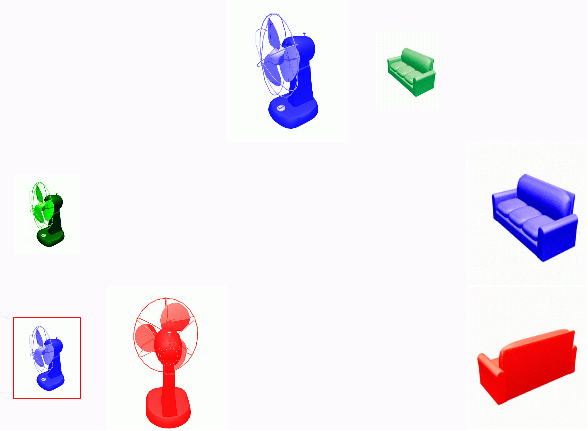
\includegraphics[width=\textwidth]{images/smallBlueFan1.jpg}
\caption{TUNA corpus people scene}
\label{smallBlueFan1}
\end{minipage}
\begin{minipage}{0.50\linewidth}
\centering
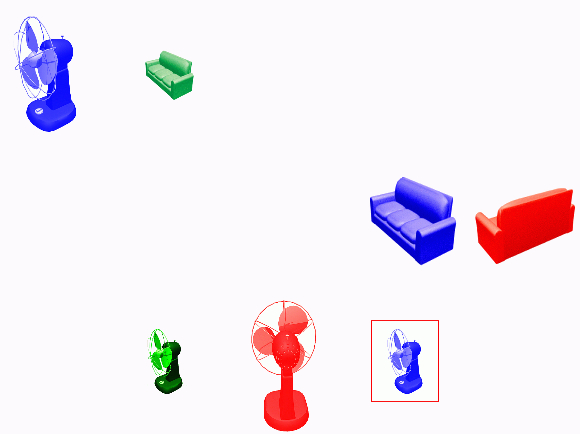
\includegraphics[width=\textwidth]{images/smallBlueFan.jpg}
\caption{TUNA corpus furniture scene}
\label{smallBlueFan}
\end{minipage}
\end{figure}

Sometimes the judges choice the human RE for example in Figure~\ref{largeGreyChair} the
system RE was ``large grey chair facing away'' and the human RE was ``the top left grey chair''.

\begin{figure}[ht]
%\begin{minipage}{0.50\linewidth}
\centering
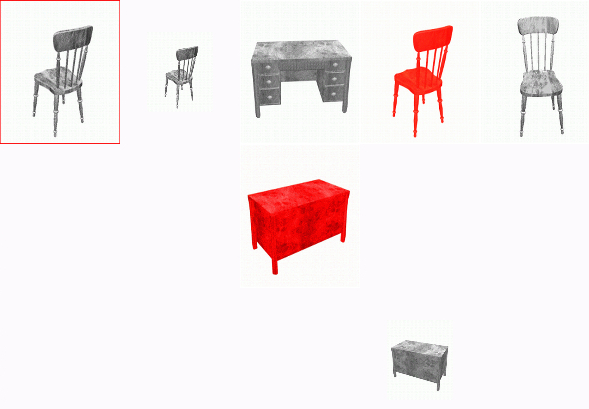
\includegraphics[width=0.8\textwidth]{images/largeGreyChair.jpg}
\caption{TUNA corpus people scene}
\label{largeGreyChair}
\end{figure}


EN HUMAN EVALUATION AGREGAR CASOS EN LOS QUE LOS JUECES CONSISTENTEMENTE ELIGIERON LA EXPRESION DE LA PERSONA Y CASOS EN LOS QUE LOS JUEVES ELIGIERON CONSISTENTEMENTE EXPRESIONES HUMANAS. DAR UNA IDEA DE PORQUE LAS EXPRESIONES DEL SISTEMA SON A VECES MEJORES Y PORQUE A VECES LAS DE LOS HUMANOS SON MEJORES (E.G. DEPENDENCIA ENTRE X E Y)
